\documentclass{article}
\usepackage{college-math-j}
\usepackage{xfrac}

%% IF YOU HAVE FONTS INSTALLED
%\usepackage{mtpro}
%\usepackage{mathtime}

\theoremstyle{theorem}
\newtheorem{theorem}{Theorem}

\theoremstyle{definition}
\newtheorem*{definition}{Definition}
\newtheorem*{remark}{Remark}

\begin{document}

\title{Visualization of [fulle name] Fractional Integrals}
\author{Woodrow Wilson and Herbert Hoover} %%leave blank in initial submission to allow for double blind reviewing
%\author{ }

\maketitle

%Notes authors should leave bios out altogether.

%\begin{biog} %comment out in initial submission to allow for double blind reviewing
%\item[\biogpic{\includegraphics[width=84pt]{Woodrow_Wilson.pdf}}Woodrow Wilson] (twwilson@princeton.edu) received his PhD in history and political science from Johns Hopkins University. He held visiting positions at Cornell and Wesleyan before joining the faculty at Princeton, where he was eventually appointed president of the university.  Among his proudest accomplishments was the abolition of eating clubs at Princeton on the grounds that they were elitist.

%\item[\biogpic{\includegraphics[width=84pt]{Herbert_Hoover.pdf}}Herbert Hoover] (hchoover@stanford.edu) entered Stanford University in 1891, after failing all of the entrance exams except mathematics.  He received his BS degree in geology in 1895, spent time as a mining engineer, then was appointed by his co-author to the U.S. Food Administration and the Supreme Economic Council, where he orchestrated the greatest famine relief efforts of all time.
%\end{biog}
%This is not to say that there  This is partly, because there is no simplistic geometric interpretation for fractional calculus.  
\noindent
Leibniz, who is regarded by many scholars as the farther of calculus, is credited with inventing the following notation: $\frac{d^n y}{d x^n}$. 
A natural question which arises when one inspects this notation is: Can $n$ be a non-integer value? L'Hospital phrased it differently: ``\emph{What if $n$ be a $\frac{1}{2}$?}''. 
In a letter Leibniz sent to L'Hospital, he himself commented on this intriguing question: ``\emph{This is an apparant paradox from which, one day, useful 
consequences will be drawn}.'' 

The mathematical discipline in which we study the extension of derivatives and integrals to non-integer orders is known as fractional calculus. Liouville and Riemann laid most 
of theoretical groundwork which was needed to develop the field of fractional calculus. Fractional calculus has now developed into a mature discipline. 
However, there is one aspect of the discipline which only started to develop fairly recently: its physical and geometric interpretability. At the first international conference on fractional calculus in
New Haven (USA) (which took place in 1974) it was pointed out that literature lacked an acceptable geometric and physical interpretation of fractional calculus. Subsequently, the last few decades has seen 
a number of papers that attempt to rectify this. There now exists probabilistic interpretations, geometric interpretations, physical interpretations and ecenomic 
interpretations of fractional order integrals and differentials. 

In this article we specifically focus on the geometric interpretation of fractional integrals. To be more specific, we present a novel geometric interpretation of the Riemann-Liouville fractional integral.
As we mentioned earlier, Riemann and Liouville played an important role in the development of fractional calculus. Their work was crucial in defining what is now know as 
the Riemann-Lioville fractional integral. At this point in time the reader should be made aware of the fact that there exists many other accepted fractional integral definitions in the literature.
We, however, do not discuss them any further in this article. Investigating whether one can apply the proposed framework to other fractional integral definitions will be adressed in a 
future endeavour.

Moreover, the geometric interpretation we present here is especially useful from a pedigogical point of view as it is similar in nature to the definition of classical integration. The Riemann integral 
can be interpreted as an infinite sum of rectangular infinitesimals. In this paper, we show that the Riemann-Liouville fractional integral can be interpreted 
as an infinite sum of non-rectangular infinitesimals whose shape is determined by the order of integration $\alpha$ and the integration limit $x$. 

The geometric interpretation we present in this paper is an extension of the fractional geometric framework presented by Podlubny. Podlubny showed that a fractional Riemann-Liouville 
integral can be converted to a Riemann-Stieltjes integral. Furthermore, Grobler showed that a Riemann-Stieltjes integral can be interpreted as an infiniesimal sum of 
non-rectangular infinitesimels, i.e. a Riemann-Stieltjes integral can be converted into a Cavalieri integral. If we combine these two ideas together we obtain the geometric interpretaion contained in the 
previous paragraph.  

We specifically wrote this paper for people with a pedagogical interest, undergraduate students and for the layman who finds integration theory intriguing and 
as such we will try to steer clear from using too many mathematical definitions and proofs. We will rather convey our ideas using as many examples as possible. From the 
three groups mentioned we believe that the undergraduate student will find this article the most useful. Although undergraduate students have a limited understanding of 
fractional calculus they generally are quite interested in the subject. This is quite evident from perusing mathematical social media platforms and from surveying 
articles published in undergraduate journals []. One of the reasons undergraduates struggle to grasp fractional calculus, apart from it not normally being taught as part of the undergraduate curricilum, is because, 
it is such an abstract concept. We believe that the geometric interpretation we present in this paper will provide undergraduates with the insight that they need to quickly grasp and understand the fundamental 
concepts that unerpin fractional calculus. We also hope that this paper will enable and encourage undergraduate lectures to already introduce students to this fascinating mathematical discipline as part of their 
undergraduate training.   

We start the paper by reviewing the definition of the Riemann-Stieltjes and Cavalieri integral. We then present the definition of the Riemann-Lioville fractional integral. 
We end the paper by presenting our novel geometric interpretation and a conclusion.

%Due to the 
%Even though most undergraduates have a limited understanding of fractional-order calculus they generally are quite interested in the subject. This is quite 
%evident from perusing mathematical social media platforms and from surveying articles published in undergraduate journals []. One of the reason fractional calculus is not generally 
%taught at the undegraduate level is due to the fact that the notion is quite abstract and it is therefore difficult to interpret geometrically. In this paper adress this shortcomming by presenting  
%a novel geometric interpretation of the Riemann-Liouville fractional integral which is similar in nature to the classical interpretation of classical integration. Our hope is that this 
%geometric interpretation will encourage and enable undergraduate lectures to introduce undergraduates to this fascinating mathematical discipline. 


%Our hope is that the geometric 
%interpretation we present here will encourage and enable undergraduate lectures to introduce undergraduates to this fascinating mathematical discipline.  


%We therefore only present the min-
%imum number of mathematical definitions that are needed to convey the new geometric framework.


%This article is not an in depth study into the field of integral calculus, but should rather be viewed as an introductory text 

%It is important to point out at this point that there exists numerous acccepted definitions of fractional integration and differentiation. For the sake of 
%simplicity we decided to focus on one In this paper we will focus 
%on the Riemann-Lioville fractional integral.

%There are many accepted definitions of fractional order differentiation and integration. In this paper we will only focus 

%In particular, their contribution played a crucial part in defining what is now known as the 
%Riemann-Lioville fractional integral. In this paper, we present a novel geometric interpretation of the Riemann-Lioville fractional integral which is similar 
%in nature to the classical interpretation of an ordinary Riemann integral. An ordinary Riemann integral can be interpreted as an infinitesimal sum of rectangular 
%infinitesimals. 

%In this paper we present a novel geometric interpretation of the Riemann-Liouville fractional integral. There are in fact many accepted definitions of fractional integration 
%The interpretation we present here is especially useful from 
%a pedigogical point of view as it is similar in nature to the definition of classical integration. as an infinite sum of rectangular infinitesimals. In this paper, we demonstrate at the hand of examples that the Riemann-Liouville fractional integral can be interpreted 
%as an infinite sum of non-rectangular infinitesimals whose shape is determined by the order of integration $\alpha$ and the integration limit $x$. Furthermore, please note that the intended audience of this 
%paper is undergraduate students and lecturers and as such we do not present .  In ordinary integration we can interpret the integral   

%Fractional calculus can be summarized as the generalization of integer-order differentiation and integration to an arbitrary order.
%Fractional-order calculus is as old as classical calculus itself. In this paper, we will mainly focus our attention on fractional-order integration and in particular investigate the Riemann-Liouville fractional 
%integral. It is Liouville and Riemann who laid much of the groundwork which was needed to define what is now known as the Riemann-Liouville fractional integral [Laurent’]. 

%The idea of integer-order differentiation and integration is well known to most undergraduates. However, undergraduates are less familiar with the idea of an arbitrary order differential or integral (i.e. fractional-order calculus).
%Even though most undergraduates have a limited understanding of fractional-order calculus they generally are quite interested in the subject. This is quite 
%evident from perusing mathematical social media platforms and from surveying articles published in undergraduate journals []. One of the reason fractional calculus is not generally 
%taught at the undegraduate level is due to the fact that the notion is quite abstract and it is therefore difficult to interpret geometrically. In this paper adress this shortcomming by presenting  
%a novel geometric interpretation of the Riemann-Liouville fractional integral which is similar in nature to the classical interpretation of classical integration. Our hope is that this 
%geometric interpretation will encourage and enable undergraduate lectures to introduce undergraduates to this fascinating mathematical discipline.  

\section{Riemann-Stieltjes Integral}
Recall that the Riemann-Stieltjes integral is defined as follows:
\begin{equation}
\label{eq:g_int2}
\int_{a'}^{b'} f(x) dg(x) =  \lim_{n \rightarrow \infty}\sum_{i=0}^{n-1} f(x_i^2)[g(x_{i+1}^2)-g(x_{i}^2)], 
\end{equation}
%Fig.~\ref{fig:2d_geo} depicts a region whose area can be determined by considering non--rectangular integration strips.
%. Note that the shape of the integration strips are determined by $a(y)$. 
%In Fig.~\ref{fig:2d_geo}, the function $a(y)$ is depicted in red. If we translate $a(y)$ along the $x$-axis we actually create two partitions on the $x$-axis, 
%i.e. $(x_i^1)_{i=0}^{n}$ and $(x_i^2)_{i=0}^{n}$ with $x_i^1\in[a,b]$ and $x_i^2\in[a',b']$.  To map partition points in $[a',b']$ to partition points 
%in $[a,b]$ we use the function $g$. The reverse is achieved through $h$. The functions $g$ and $h$ depend soly on $a(y)$ and are also 
%computed with it.
\noindent
\textbf{NEED TO REWRITE SOME OF IT} with $(x_i^2)_{i=0}^n$ being arbitrary partition points on the $x$-axis. Eq.~\eqref{eq:g_int2} shows us that the function of the integrator $g$ is to
map points in the interval $[a',b']$ to other locations on the $x$-axis. When $g$ is monotone increasing, it maps points in the interval $[a',b']$ to $[a,b]$,
with $a = g(a')$ and $b = g(b')$. The integral in Equation~\ref{eq:g_int2} is hard to evaluate in its present form. If $g$ is differentiable, however, then it becomes trivial to 
evaluate a Riemann-Stieltjes integral due to the following identity:
\begin{equation}
\int_{a'}^{b'} f(x) dg(x) = \int_{a'}^{b'} f(x)g'(x)~dx.
\end{equation}
As an example:
\begin{equation}
\int_{\frac{1}{2}}^{2} f(x) dg(x)=\int_{\frac{1}{2}}^2 x~d2x = \int_{\frac{1}{2}}^2 2x~dx = 3.75. 
\end{equation}

\section{Cavalieri Integral}
Let the region $R$ be bounded by the $x$-axis and the lines $f(x)=x$, $a(y)=1-y$ and $b(y)=4-y$. This region is shown in Fig.~\ref{fig:caval2}.\\
%\begin{figure}[htb]
%\centering
%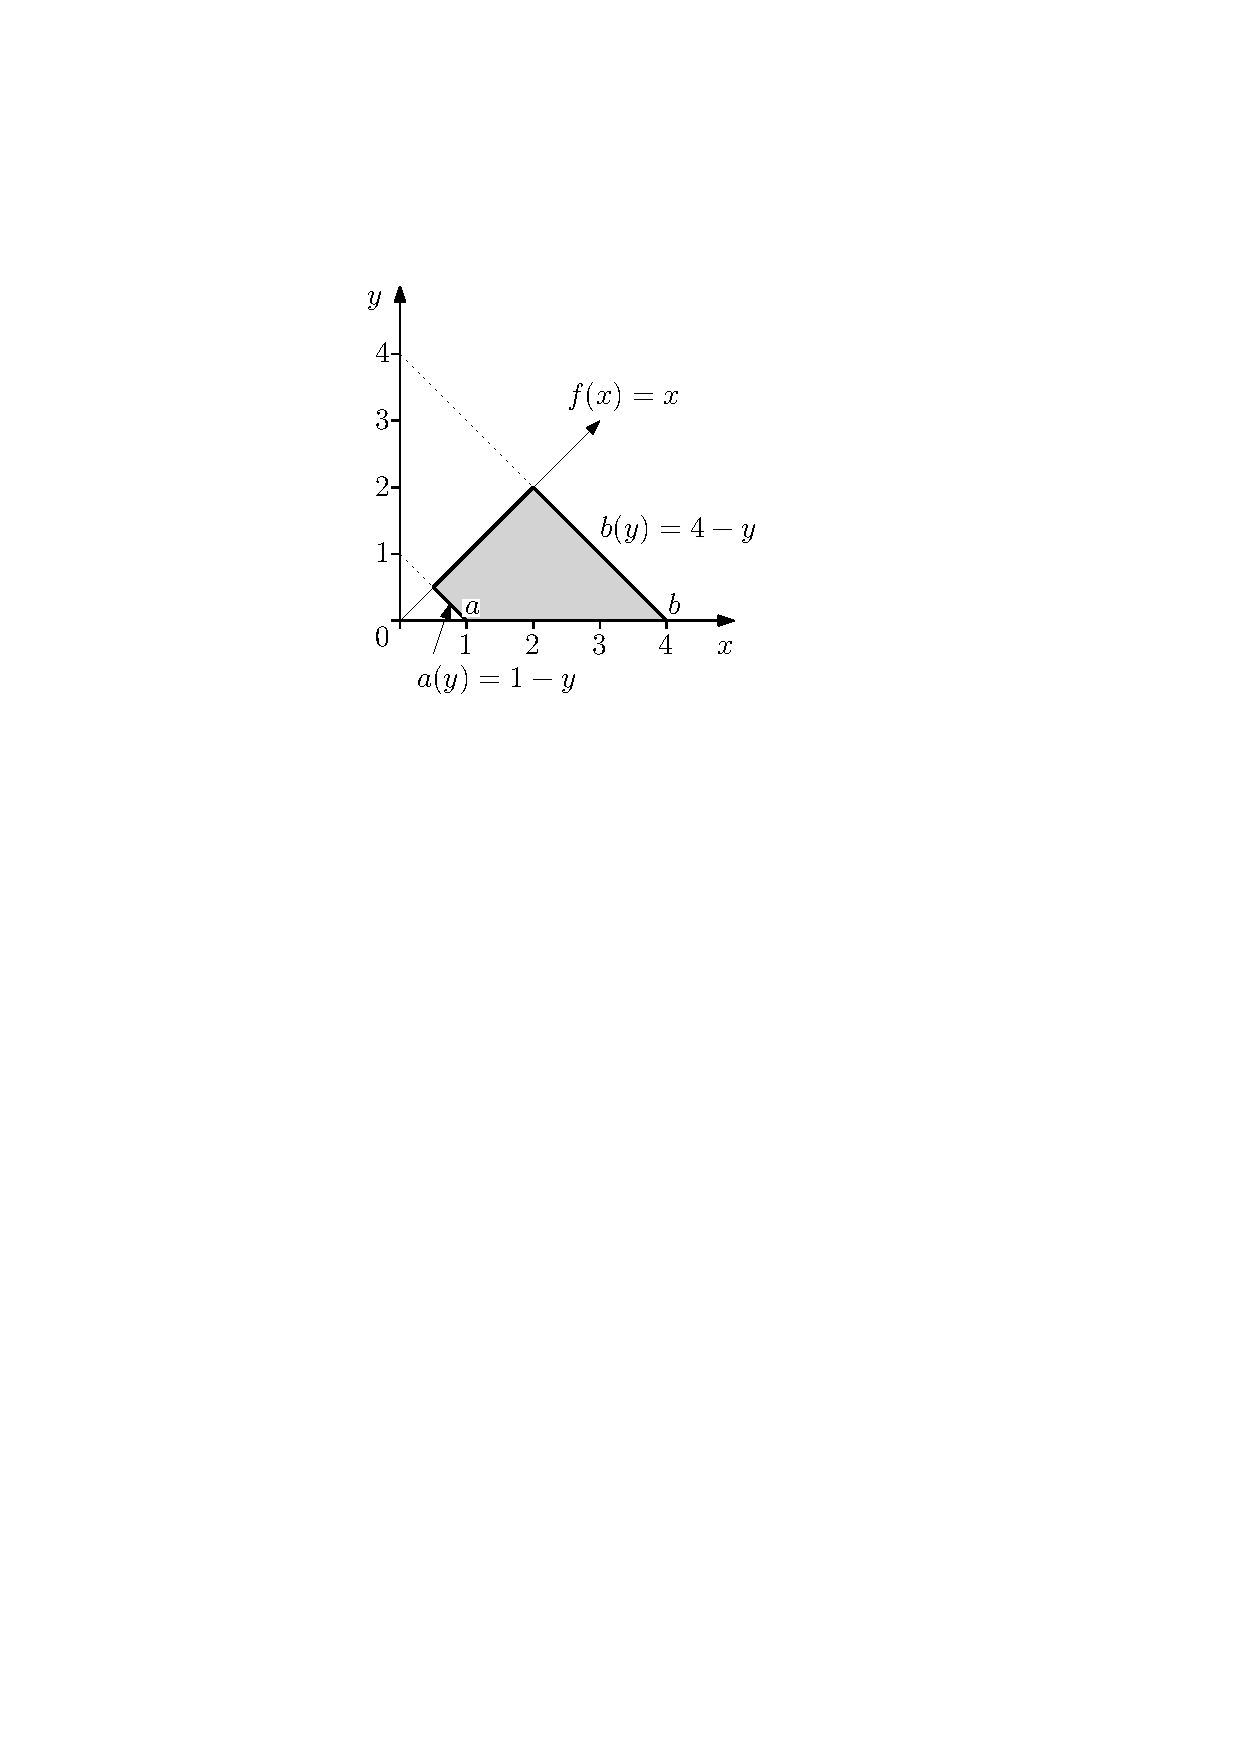
\includegraphics[width=0.3\textwidth]{fig12}
%\caption{Region bounded by the $x$-axis and the lines $f(x)=x$, $a(y)=1-y$, and $b(y)=4-y$. Reproduced from Quaestiones Mathematicae (2012) 35: 265-296 with permission \copyright~ NISC (Pty) Ltd.}
%\label{fig:ex1}
%\end{figure}
\begin{figure}[htb]
\centering
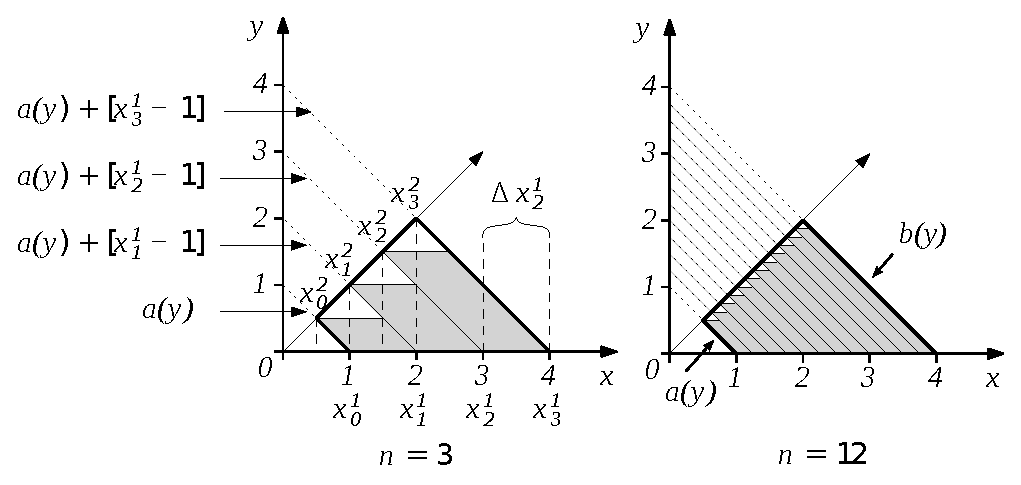
\includegraphics[width=0.75\textwidth]{fig13.eps}
\caption{Region bounded by the $x$-axis and the lines $f(x)=x$, $a(y)=1-y$, and $b(y)=4-y$. The figure also depicts the partition points $x_i^2$ as used in the Cavalieri sum (see Eq.~\ref{eq:cav_sum}). Reproduced from Quaestiones Mathematicae (2012) 35: 265-296 with permission \copyright~ NISC (Pty) Ltd.}
\label{fig:caval2}
\end{figure}

\noindent
The area of $R$ can be determined as follows if we employ the classical notion of integration:
\begin{equation}
\int_0^2x\, dx+\int_2^44-x\, dx- \int_0^{\frac{1}{2}}x\, dx-\int_{\frac{1}{2}}^11-x\, dx = 3.75. 
\end{equation}

There, however, exists a more straightforward way do determine the area of $R$, i.e. we can sum together the area of non-rectangular integration strips inscribing $R$ instead of
having to sum together the area of multiple rectangular integration strips. Moreover, the shape of the non-rectangular integration strips we should use is determined by the function $a(y)$. We can express this notion more formally as 
follows, let $(x_i^1)_{i=0}^{n}$ denote a partition on the $x$-axis, such that $a = x_0^1 < x_1^1 < \cdots < x_n^1 = b$, and $\Delta x_i^1 = x_{i+1}^1 - x_i^1$.
We are now able to construct the following sum (the lower Cavalieri sum):
\begin{equation}
\label{eq:cav_sum}
\sum_{i=0}^{n-1} f(x_i^2)\Delta x_i^1.
\end{equation}
The partition points $(x_i^2)_{i=0}^{n}$ are depicted in Fig.~\ref{fig:caval2}. Note that Equation~\ref{eq:cav_sum} approximates the area of $R$. In the limit Equation~\ref{eq:cav_sum} approaches 
the Cavalieri integral:
\begin{equation}
\label{eq:caval1}
\int_{a(y)}^{b(y)}f(x)\, dx = \lim_{n\to \infty}\sum_{i=0}^{n-1} f(x_i^2)\Delta x_i^1.
\end{equation}
It is, however, quite hard to evaluate the above integral directly. Fortunately, it is easy to convert a Cavalieri integral into an equivalent Riemann or Riemann-Stieltjes 
integral by using the transformation functions $h$ and $g$. Expressed mathematically:
\begin{equation}
\int_{a(y)}^{b(y)}f(x)\,dx =\int_a^b f \circ h (x)\, dx = \int_{a'}^{b'} f(x) dg(x).
\end{equation}
We can calculate $g$ as follows:
\begin{equation}
g(x) = x - a\circ f(x) + a.
\end{equation}
Moreover, $h=g^{-1}$. We can now evaluate the Cavalieri integral by using its equivalent Riemann or Rieman-Stieltjes integral.
If we use its Riemann equivalent we obtain:
\begin{equation}
\int_{a(y)}^{b(y)}f(x)\, dx = \int_a^b f \circ h (x)\, dx = \dfrac{1}{2}\int_1^4x\, dx = 3.75.  
\end{equation}
If we use its Riemann-Stieltjes equivalent we obtain:
\begin{equation}
\int_{a(y)}^{b(y)}f(x)\, dx = \int_{a'}^{b'} f \, dg(x) = \int_{\frac{1}{2}}^2x\, d2x = 3.75.  
\end{equation}

Conversely, if $g$ is known (and not $a(y)$) and $g(a') = a$ then we can calculate $a(y)$ using the following:
\begin{equation}
\label{eq:a_y}
a(y) = f^{-1}(y) - g\circ f^{-1}(y) + g(a'). 
\end{equation}
Note the power of Equation~\ref{eq:a_y} it allows us to transform a Riemann-Stieltjes integral into a Cavalieri integral. 
This transformation allows us to give a geometric interpretation of a Riemann-Stieltjes integral. The interpretation being,
the sum of an infinite amount of non-rectangular infinitesimals whose shape is determined by $a(y)$.

\section{Gamma Function}
The gamma function was first devised by Euler. The gamma function is defined for all real numbers except for the non-negative integers. Moreover, it is a natural extension of the factorial function to the real numbers. The Gamma function is defined as:
\begin{equation}
\Gamma(x) = \int_0^{\infty} t^{x-1} e^{-t}\,dt
\end{equation}
\begin{figure}[htb]
\centering
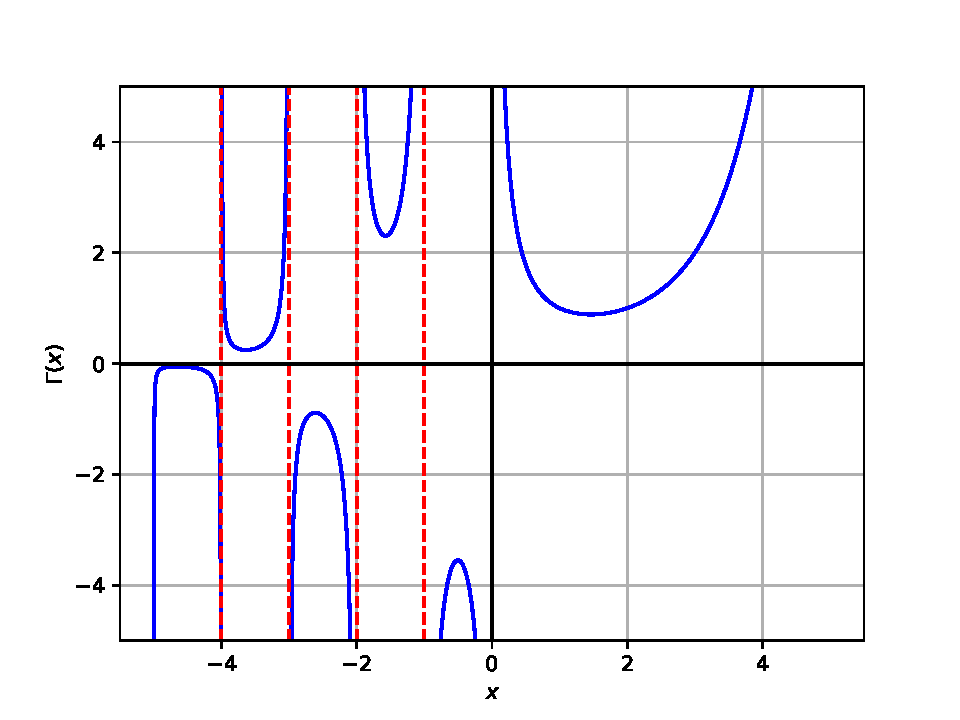
\includegraphics[width=0.75\textwidth]{gamma.pdf}
\caption{A plot of $\Gamma(x)$. $\Gamma(x)$ is not defined for the non-negative integers.}
\label{fig:gamma}
\end{figure}



\section{Riemann-Liouville Fractional Integral}
In this section we derive the definition of the Riemann-Liouville fractional integral of order $\alpha$. Let
\begin{equation}
If(x) := \int_0^x f(t) dt.
\end{equation}
If we apply the above operator in a repetative manner to $f$ we obtain the $n$th antiderivative of $f$ based at 0:
\begin{equation}
\label{eq:n_anti}
I^nf(x) = \int_0^x\int_0^{x_1}\cdots \int_0^{x_{n-1}}f(x_n)~dx_n\cdots dx_2 dx_1.
\end{equation}
Applying Cauchy's formula for repetative integration to the above $n$th antiderivative of $f$ helps us express the above $n$th antiderivative as a single integral. 
Applying Cauchy's formula to Equation~\ref{eq:n_anti} results in:
\begin{equation}
\label{eq:cauchy}
I^nf(x) = \frac{1}{(n-1)!}\int_0^x (x-t)^{n-1}f(t)~dt.
\end{equation}
As an example if $f(x)=x$ and $n=2$ then Equation~\ref{eq:cauchy} reduces to:
\begin{equation}
I^2f(x) = \int_0^x (x-t)t~dt = \frac{t^2x}{2} - \frac{t^3}{3} \Bigg |_0^x = \frac{x^3}{3!}.
\end{equation}
The definition in Equation~\ref{eq:cauchy} can now be extended to an arbitrary fractional order by replacing $(n-1)!$ with the Gamma function:
\begin{equation}
\label{eq:frac_integral}
I^{\alpha}f(x) = \frac{1}{\Gamma(\alpha)}\int_0^x (x-t)^{\alpha-1}f(t)~dt.
\end{equation}
Equation~\ref{eq:frac_integral} is known as the Riemann-Liouville fractional integral of order $\alpha$. As an example if $f(x)=x$ and $\alpha=\frac{1}{2}$ then 
Equation~\ref{eq:frac_integral} reduces to:
\begin{equation}
I^{\frac{1}{2}}f(x) = \frac{1}{\Gamma(\frac{1}{2})} \int_0^x \frac{t}{\sqrt{x-t}} dt = \frac{1}{\sqrt{\pi}}\left [ -\frac{2}{3}\sqrt{x-t}(t+2x)\right] \Bigg |_0^x=\frac{4}{3\sqrt{\pi}}x^{\frac{3}{2}}. 
\end{equation}
Furthermore, it is straightforward to show that the $I$ operator satisfies:
\begin{equation}
I^{\alpha}I^{\beta}f(x) = I^{\alpha+\beta}f(x). 
\end{equation}

\section{Geometric Interpretation of the Riemann-Liouville Fractional Integral}

Recall that the Riemann-Liouville fractional integral of order $\alpha$ is defined as:
\begin{equation}
\label{eq:RL_frac_int}
\frac{1}{\Gamma(\alpha)}\int_{0}^{t}f(\tau)(t-\tau)^{\alpha-1}~d\tau
\end{equation}

Podlubny showed that the above fractional integral can be rewritten as a Riemann-Stieltjes integral:
\begin{equation}
\label{eq:rs}
\int_0^{t} f(\tau)~dg_t(\tau),
\end{equation}
with 
\begin{equation}
g_t^{\alpha}(\tau) = \frac{\left \{t^{\alpha} - (t-\tau)^{\alpha} \right \}}{\Gamma(\alpha+1)}. 
\end{equation}

Note that $g_t^{\alpha}(\tau)$ is always invertable, since $\frac{d g_t^{\alpha}}{d \tau} = \frac{(t-\tau)^{\alpha-1}}{\Gamma(\alpha)}>0$ for $\tau\in[0,t]$. The inverse 
of $g_t^{\alpha}(\tau)$ is equal to:
\begin{equation}
h_t^{\alpha}(x) = t - \sqrt[\alpha]{t^{\alpha} - \Gamma(\alpha+1)x}
\end{equation}

Let $\mathsf{A} = \{0,0.2,0.4,0.6,0.8,1\}$. The analytic expressions of $g_t^{\alpha}(\tau)$ and $h_t^{\alpha}(x)$ are presented in Table~\ref{eq:} for $\alpha\in\mathsf{A}$ and $t=10$. 
The expressions in Table~\ref{eq:} are depicted in Fig~\ref{fig:}.

Grobler et. al showed that it is trivial to convert a Riemann-Stieltjes integral into a Cavalieri integral. We review this conversion procedure in the Cavalieri section of this paper. Applying their approach to Eq.~\ref{eq:rs} results in:
\begin{equation}
\label{eq:cav}
\int_{a_t^{\alpha}(y)}^{b_t^{\alpha}(y)} f(\tau)~d\tau, 
\end{equation}
with
\begin{equation}
a_t^{\alpha}(y) = f^{-1}(y) - \frac{t^{\alpha}-(t-f^{-1}(y))^{\alpha}}{\Gamma(\alpha+1)}.
\end{equation}
Note, Eq.~\eqref{} is obtained by substituting Eq.~\eqref{} into Eq.~\eqref{}.

Since Equation~\ref{eq:cav} is a Cavalieri integral, it has a clear geometric interpretation. The integral in Equation~\ref{eq:RL_frac_int} can, therefore, be interpreted as the area obtained 
by summing toghether the area of an infinite number of infinitesimally small non–rectangular integration strips whose shape is determined by $\alpha$ and $t$. The shape of the integration 
strip will change if either $\alpha$ or $t$ is changed. If $\alpha$ is equal to one, however, then the integral reduces to a normal Riemann integral as the integration strips become rectangular for this particular choice of $\alpha$ (its shape is now also no longer affected by $t$).

Furthermore, Eq.~\eqref{??} implies that we can use $h_t^{\alpha}(x)$ to convert Eq.~\eqref{eq:cav} into the following Riemann integral:
\begin{equation}
\int_0^{\frac{t^{\alpha}}{\Gamma(\alpha+1)}} f\circ h_{\alpha}^t (\tau) d\tau.  
\end{equation}
We can, therefore, evaluate Eq.~\eqref{eq:cav} in one of two ways: we can either evaluate Eq.~\eqref{} or we can evaluate Eq.~\eqref{}.


\begin{table}[h!]
\centering
 \begin{tabular}{|c || c | c|} 
 \hline
 $\alpha$ & $g_{10}^{\alpha}(\tau)$ & $h_{10}^{\alpha}(\tau)$ \\ [0.5ex] 
 \hline\hline
 $0$ & 0 & $y=0$ \\ 
 $0.2$ & $[\Gamma\left (\frac{6}{5} \right )]^{-1}\left(\sqrt[5]{10}-\sqrt[5]{10-\tau}\right)$ & $10 - \left ( \sqrt[5]{10} -  \Gamma\left (\frac{6}{5} \right ) \tau \right )^5$  \\
 $0.4$ & $[\Gamma\left (\frac{7}{5} \right )]^{-1}\left(\sqrt[5]{10^2}-\sqrt[5]{(10-\tau)^2}\right)$ & $10 - \sqrt{\left ( \sqrt[5]{10} -  \Gamma\left (\frac{7}{5} \right ) \tau \right )^5}$ \\
 $0.6$ & $[\Gamma\left (\frac{8}{5} \right )]^{-1}\left(\sqrt[5]{10^3}-\sqrt[5]{(10-\tau)^3}\right)$ & $10 - \sqrt[3]{\left ( \sqrt[5]{10} -  \Gamma\left (\frac{8}{5} \right ) \tau \right )^5}$ \\
 $0.8$ & $[\Gamma\left (\frac{9}{5} \right )]^{-1}\left(\sqrt[5]{10^4}-\sqrt[5]{(10-\tau)^4}\right)$ & $10 - \sqrt[4]{\left ( \sqrt[5]{10} -  \Gamma\left (\frac{9}{5} \right ) \tau \right )^5}$ \\ [1ex] 
 $1$ & $\tau$ & $\tau$ \\ [1ex] 
 \hline
 \end{tabular}
\end{table}

\begin{table}[h!]
\centering
 \begin{tabular}{|c || c | c|} 
 \hline
 & \multicolumn{2}{|c|}{$a_{10}^{\alpha}(\tau)$}\\
 \hline
 &$f(\tau) = \tau$ & $f(\tau)=\sqrt{\tau}$ \\ [0.5ex] 
 \hline\hline
 $0$ & 0 & $y=0$ \\ 
 $0.2$ & $y-[\Gamma\left (\frac{6}{5} \right )]^{-1}\left(\sqrt[5]{10}-\sqrt[5]{10-y}\right)$ & $y^2-[\Gamma\left (\frac{6}{5} \right )]^{-1}\left(\sqrt[5]{10}-\sqrt[5]{10-y^2}\right)$  \\
 $0.4$ & $y-[\Gamma\left (\frac{7}{5} \right )]^{-1}\left(\sqrt[5]{10^2}-\sqrt[5]{(10-y)^2}\right)$ & $y^2-[\Gamma\left (\frac{7}{5} \right )]^{-1}\left(\sqrt[5]{10^2}-\sqrt[5]{(10-y^2)^2}\right)$ \\
 $0.6$ & $y-[\Gamma\left (\frac{8}{5} \right )]^{-1}\left(\sqrt[5]{10^3}-\sqrt[5]{(10-y)^3}\right)$ & $y^2-[\Gamma\left (\frac{8}{5} \right )]^{-1}\left(\sqrt[5]{10^3}-\sqrt[5]{(10-y^2)^3}\right)$ \\
 $0.8$ & $y-[\Gamma\left (\frac{9}{5} \right )]^{-1}\left(\sqrt[5]{10^4}-\sqrt[5]{(10-y)^4}\right)$ & $y^2-[\Gamma\left (\frac{9}{5} \right )]^{-1}\left(\sqrt[5]{10^4}-\sqrt[5]{(10-y^2)^4}\right)$ \\ [1ex] 
 $1$ & $\tau$ & $\tau$ \\ [1ex] 
 \hline
 \end{tabular}
\end{table}

\begin{table}[h!]
\centering
 \begin{tabular}{|c || c|} 
 \hline
 Symbol & Definition  \\ [0.1ex]
 \hline 
 \rule{0pt}{2.5ex}
 $\mathsf{G}^{10}$ & $\{g_{10}^{\alpha}(\tau)|\alpha\in\{0,\frac{1}{5},\frac{2}{5},\frac{3}{5},\frac{4}{5}\}\}$\\ [0.5ex]
 $\mathsf{H}^{10}$ & $\{h_{10}^{\alpha}(\tau)|\alpha\in\{0,\frac{1}{5},\frac{2}{5},\frac{3}{5},\frac{4}{5}\}\}$\\ [0.5ex]
 $\mathsf{A}^{10}$ & $\{a_{10}^{\alpha}(\tau)|\alpha\in\{0,\frac{1}{5},\frac{2}{5},\frac{3}{5},\frac{4}{5}\}\}$\\ [0.5ex]
 $\mathsf{B}^{10}$ & $\{b_{10}^{\alpha}(\tau)|\alpha\in\{0,\frac{1}{5},\frac{2}{5},\frac{3}{5},\frac{4}{5}\}\}$\\ [0.5ex]
 $\mathsf{B}^{\frac{4}{5}}_1$ & $\{b_{t}^{\frac{4}{5}}(\tau)|t\in\alpha\in\{2,4,6,8,10\}$\\ [0.5ex]
 $\mathsf{B}^{\frac{4}{5}}_2$ & $\{b_{10}^{\frac{4}{5}}(\tau)-c|c\in\in\{0,2,4,6,8\}$\\ [0.5ex]
 \hline 
 \end{tabular}
\end{table}


\begin{table}[h!]
\centering
 \begin{tabular}{||c|| c| c||} 
 \hline
 $\alpha$ & $\frac{1}{\Gamma(\alpha)}\int_0^t \tau(t-\tau)^{\alpha-1}~d\tau$ & $\frac{1}{\Gamma(\alpha)}\int_0^t \sqrt{\tau}(t-\tau)^{\alpha-1}~d\tau$ \\[0.5ex]
 \hline\hline
 \rule{0pt}{2.5ex}
 $0$ & $t$ & $\sqrt{t}$  \\  
 \rule{0pt}{2.5ex}
 $0.2$ & $\frac{25}{6\Gamma(\frac{1}{5})} t^{\frac{6}{5}}$  & $\frac{\sqrt{\pi}}{2\Gamma(\frac{17}{10})} t^{\frac{7}{10}}$  \\ 
 \rule{0pt}{2.5ex}
 $0.4$ & $\frac{25}{14\Gamma(\frac{2}{5})} t^{\frac{7}{5}}$  & $\frac{\sqrt{\pi}}{2\Gamma(\frac{19}{10})} t^{\frac{9}{10}}$  \\
 \rule{0pt}{2.5ex}
 $0.6$ & $\frac{25}{24\Gamma(\frac{3}{5})} t^{\frac{8}{5}}$  & $\frac{\sqrt{\pi}}{2\Gamma(\frac{21}{10})} t^{\frac{11}{10}}$  \\ 
 \rule{0pt}{2.5ex}
 $0.8$ & $\frac{25}{36\Gamma(\frac{4}{5})} t^{\frac{9}{5}}$  & $\frac{\sqrt{\pi}}{2\Gamma(\frac{23}{10})} t^{\frac{13}{10}}$  \\ 
 \rule{0pt}{2.5ex}
 $1$ & $\frac{1}{2}t^2$  & $\frac{2}{3}t^{\frac{3}{2}}$  \\ [1ex]
 \hline
 \end{tabular}
\end{table}

\section{Examples}
In this section we will illustrate the usefulness of the proposed geometric framework at the hand of two examples.

Let us first consider the following fractional integral:
\begin{equation}
\label{eq:ex1_raw}
\frac{1}{\Gamma(\alpha)}\int_0^t f(\tau) (t-\tau)^{\alpha-1}~d\tau = \frac{1}{\Gamma(\alpha)}\int_0^t \tau(t-\tau)^{\alpha-1}~d\tau. 
\end{equation}
The function $f(\tau) =\tau$ is depicted in Figure~\ref{??}. As we mentioned in the previous section, we can assign a geometric interpretation to the above fractional integral by converting it into a Cavalieri integral using two steps. First, we convert 
the above integral into a Riemann-Stieltjes integral:
\begin{equation}
\frac{1}{\Gamma(\alpha)}\int_0^t f(\tau) (t-\tau)^{\alpha-1}~d\tau = \int_0^t f(\tau)~dg_t^{\alpha}(\tau). 
\end{equation}
We then convert the resulting Riemann-Stieltjes integral into a Cavalieri integral:
\begin{equation}
\label{eq:ex1}
\frac{1}{\Gamma(\alpha)}\int_0^t f(\tau) (t-\tau)^{\alpha-1}~d\tau = \int_0^t f(\tau)~dg_t^{\alpha}(\tau)=\int_{a_t^{\alpha}(y)}^{b_t^{\alpha}(y)} f(\tau)~d\tau. 
\end{equation}

As we mentioned in the previous section Eq.~\ref{eq:ex1} has a clear geometric interpretation. It can be interpreted as the area obtained by summing togheher the areas of an infinite 
number of infinitesimals whose shape is determined by $\alpha$ and $t$. The thing which remains unclear, however, is in what way does $\alpha$ and $t$ affect the 
shape of the aforementioned infinitesimals. We will this question using two steps: we will first investigate the shape of the infinitesimal we obtain by fixing 
$\alpha$ and $t$ to specific values. We will then explore how varying the value of $\alpha$ and $t$ affects the shape of the infinitesimals.

%We know that a Cavalieri integral can be interpreted as the area which is obtained by summing together the area associated with an infinite number of non-rectangular infinitesimals whose shape 
%is determined by the integration limits of the Cavalieri integral. Note that neither $g_t^{\alpha}(\tau)$ nor $a_t^{\alpha}(y)$ are static functions, 
%they depend on the value of $\alpha$ and $t$. This implies that a fractional integral of order $\alpha$ and extent $t$ can be interpeted as the area obtained by summing together the area associated with an infinite number of infinitesimals whose 
%shape is determined by $\alpha$ and $t$, i.e. the geometric interpretation of Eq.~\eqref{eq:ex1_raw} is non-static as it depends on the value of $\alpha$ and $t$.

If we set the value of $\alpha$ to $\sfrac{4}{5}$ and the value of $t$ to 10 in Eq.~\eqref{eq:ex1} we obtain:
\begin{equation}
\label{eq:ex1_specific}
A_{10}^{\sfrac{4}{5}}=\int_{a_{10}^{\frac{4}{5}}(y)}^{b_{10}^{\frac{4}{5}}(y)} f(\tau)~d\tau 
\end{equation}
Let $R_{10}^{\sfrac{4}{5}}$ denote the region which is bounded by the $\tau$-axis, the function $f(\tau)$ and the function $b_{10}^{\sfrac{4}{5}}(y)$. The region $R_{10}^{\sfrac{4}{5}}$ is depicted and labelled in the right-most panel of Figure.~\ref{??}. 
Moreover, let $A_{10}^{\sfrac{4}{5}}$ denote the area of $R_{10}^{\sfrac{4}{5}}$. We can approximate the area of $R_{10}^{\sfrac{4}{5}}$ by summing together the area of $n$ equal width non-rectangular integration strips that inscribe $R_{10}^{\sfrac{4}{5}}$. 
Furthermore, the sides of the non-rectangular integration strips we use in this approximation have to be translations of $b_{10}^{\sfrac{4}{5}}(y)$.
If we take the limit of the aforementioned sum as $n\rightarrow \infty$ we obtain $A_{10}^{\sfrac{4}{5}}$, i.e. if we evaluate the Cavalieri 
integral in Eq.~\eqref{??} we obtain $A_{10}^{\sfrac{4}{5}}$ (as we mentioned in the previous section). We can, therefore, think of Eq.~\eqref{} as implying that that the region  $R_{10}^{\sfrac{4}{5}}$ is made up 
of an infinite number of non-rectangular infinitesimals; all of them being translations of $b_{10}^{\sfrac{4}{5}}(y)$. Moreover, the special case in which we approximate $A_{10}^{\sfrac{4}{5}}$ using five equal width non-rectangular integration strips is depicted in the right-most panel of Figure~\ref{??}. 
The sides of the aforementioned five integration strips are depicted in Fig.~\ref{??} using dashed lines. Let $\mathsf{B}_{10}^{\sfrac{4}{5}}$ denote the set containing these dashed curves.

%We can, therefore, interpet Eq.~\eqref{}  The region $R_{10}^{\sfrac{4}{5}}$ is, therefore, made up 
%of an infinite number of non-rectangular infinitesimals; all of them being translations of $b_{10}^{\sfrac{4}{5}}(y)$.

Varying both $\alpha$ and $t$ results in Eq.~\eqref{eq:ex1}. In contrast with Eq.~\eqref{eq:ex1_specific}, Eq.~\eqref{eq:ex1} can be associated with more than one region. 
Let $R_{t}^{\alpha}$ denote the region which is bounded by the $\tau$-axis, the function $f(\tau)$ and the function $b_{t}^{\alpha}(y)$. Moreover, let $A_{t}^{\alpha}$ denote the area of $R_{t}^{\alpha}$ and let $\mathsf{R}_{\mathsf{T}}^{\mathsf{A}}=\{R_t^{\alpha}|t\in\mathsf{T},~\alpha\in\mathsf{A}\}$. 
The regions in the set $\mathsf{R}_{\mathsf{T}}^{\mathsf{A}}$ are depicted in Fig.~\textbf{??}. The regions that are depicted in each of the panels of Fig.~\ref{??} were generated by varying $t$, whilst keeping the value of $\alpha$ fixed. 
The title of each panel indicate which $\alpha$-value was used to generate the regions depicted in each panel. The only difference between the regions located in each 
panel is their right edges. The right edges of the regions in each panel are depicted using varying shades of gray. The lighter the shade with which an edge is depicted, 
the larger the $t$-value is, that was used to generate it.

As was the case for $R_{10}^{\sfrac{4}{5}}$, each of the regions depicted in Fig.~\ref{} are made up of an infinite number of infinitesimals. The infinitesimals that make up a specific region are translations of that region's right edge. 
The following observations can be made by inspecting Fig.\ref{??}: 
\begin{description}
 \item[Effect of $\alpha$] the grey-tinted solid curves depicted in the different panels of Fig.~\ref{} are not equal to one-another.
 \item[Effect of $t$] the grey-tinted solid curves depicted in each of the panels of Fig.~\ref{} are not translations of one-another. Moreover, the dashed grey curves and the solid grey-tinted curves in the right-most panel are not equal to one-another.
\end{description}
We can therefore draw the following conclusion: the value of both $\alpha$ and $t$ alters the shape of the infinitesimals that make up the regions in Fig~\ref{??}. Interestingly, the effect of $\alpha$ on the shape of the infinitesimals that make up the regions depicted in Fig~\ref{??} is larger than the effect that $t$ has on their shape. 
The curves associated with the infinitesimals obtained by varying $t$, whilst keeping the value of $\alpha$ fixed are very similar in nature and there exists a high degree of correlation between them (if their 
size are ignored). The curves associated with the infinitesimals obtained by varying $\alpha$, whilst keeping the value of $t$ fixed are quite different from one another (the aforementioned curves are not highly correlated with 
one another).  

%In the case of $\alpha$: the grey-tinted solid curves depicted in each panel are not equal to one-another. Similarly, in the case of $t$: the dashed grey curves and the solid grey-tinted curves in the right-most panel are not equal to one-another, i.e.$\mathsf{B}_T^{\alpha}\neq\mathcal{B}_T^{\alpha}$.

If we evaluate the integral in Eq.~\eqref{eq:ex1} for all $\alpha\in \mathsf{A}$ we obtain the curves in the left-most column of Table~\ref{??}. These curves are depicted in Fig~\ref{??}.
The area of the regions depicted in Fig.~\ref{??} are also plotted in Fig.~\ref{??} using circular markers. As expected, the circular markers in Fig.~\ref{??} that correspond to the areas of the regions in Fig.~\ref{??}  
associated with a particular choice of $\alpha$ (i.e. regions depicted in a particular panel of Fig.~\ref{??}) fall on the curve in Fig.~\ref{??}; associated with the same choice of $\alpha$. Moreover, note that we have adopted the 
same coloring scheme in Fig.~\ref{??} and Fig.~\ref{??}. Using the same coloring scheme in both figures makes it clear which of the area values in Fig.~\ref{??} can be associated with which regions in Fig.~\ref{??}.
To summarize, Fig.~\ref{??}, therefore, depicts a non-static non-rectangular sum-based geometric interpretation of Eq.~\eqref{}. Moreover, Fig.~\ref{??} corroborates this 
geometric interpretation.

Let us know consider a different fractional integral:
\begin{equation}
\frac{1}{\Gamma(\alpha)}\int_0^t f(\tau) (t-\tau)^{\alpha-1}~d\tau = \frac{1}{\Gamma(\alpha)}\int_0^t \sqrt{\tau}(t-\tau)^{\alpha-1}~d\tau. 
\end{equation}
If we evaluate the integral in Eq.~\eqref{eq:ex1} for all $\alpha\in \mathsf{A}$ we obtain the curves in the right-most column of Table~\ref{??}. These curves are depicted in Fig~\ref{??}.
The non-static non-rectangular sum-based geometric interpretation associated with Eq.~\eqref{eq:ex1} is depicted in Fig. The validity of this interpretation is corroborated by Fig. 

To conclude this section, a fractional integral of order $\alpha$ and extent $t$ can be interpreted as the area obtained by summing together the area associated with an infinite number of infinitesimals whose 
shape is determined by $\alpha$ and $t$. The geometric interpretation of a fractional integral is, therefore, non-static as it depends on the value of both $\alpha$ and $t$. 

%the fractional integral in Eq.~\ref{??} can be interpreted as the area which is obtained by summing together the area associated with an infinite number of non-rectangular infinitesimals whose shape 
%is determined by the integration limits of the Cavalieri integral. Note that neither $g_t^{\alpha}(\tau)$ nor $a_t^{\alpha}(y)$ are static functions, 
%they depend on the value of $\alpha$ and $t$. This implies that a fractional integral of order $\alpha$ and extent $t$ can be interpeted as the area obtained by summing together the area associated with an infinite number of infinitesimals whose 
%shape is determined by $\alpha$ and $t$, i.e. the geometric interpretation of Eq.~\eqref{eq:ex1_raw} is non-static as it depends on the value of $\alpha$ and $t$.



The circular markers in Figure ?? is depicted using the same tint-of-gray with which the right edge of the region  in question is depicted in Fig.



Each of the curves 
in Fig can therefore be associated with one of the panels in Fig. The area associated with the regions depicted in each of the panels in Fig. are plotted on the curves 
in 
associated with a particular panel appropriate 
curves 
in Fig using circular markers. The circular marker is depicted in Figure using the same tint-of-gray with which the 
right edge of the region in question is depicted in Fig.  

it is $\alpha$  
Although $\alpha$ and $t$ alters the shape of the infinitesimals which make up the regions depicted in Fig.,  

that make up the regions in Fig are confirmed by the following observation: $\mathsf{B}_T^{\alpha}\neq\mathcal{B}_T^{\alpha}$.
We can visually verify that this observation is in fact true for $alpha=\frac{4}{5}$ by inspecting the right-most panel in Fig.~\ref{??}. The dashed curves and the grey tinted curves in this panel do not allign.



the upper limit 
of the Cavalieri integral in Eq. As the upper limit of the Cavalieri integral depends on

As the shape of the infinitesimals which make up the regions depicted in Fig depend of the integration limit of the 
Cavalieri integral or stated differently on the value of $t$ and $\alpha$.  

If we set the value of $\alpha$ to $\frac{4}{5}$, but we do not fix the value of $t$ then Eq.~\eqref{eq:ex1} reduces to:
\begin{equation}
\int_{a_{t}^{\frac{4}{5}}(y)}^{b_{t}^{\frac{4}{5}}(y)} f(\tau)~d\tau 
\end{equation}
If we evaluate the above integral we obtain the area of the region $R_{t}^{\frac{4}{5}}$. The region $R_{t}^{\frac{4}{5}}$ is the region bounded by the $\tau$-axis, the function $f(\tau)$ and the function $b_{t}^{\frac{4}{5}}(y)$.
Note that the shape of $R_{t}^{\frac{4}{5}}$ depends on the value of $t$. The regions contained in the set $\mathsf{R}^{\frac{4}{5}}$ are depicted in the rightmost panel of Fig\textbf{??}. Let $\mathsf{B}^{\frac{4}{5}}$ contain the right 
edges of the regions contained in the set $\mathsf{R}^{\frac{4}{5}}$. The shape of the edges in $\mathsf{B}^{\frac{4}{5}}$ depend on the value of $t$. The edges in $\mathsf{B}^{\frac{4}{5}}$ are depicted in Fig?? using different shades of gray. The shade with which the aformentioned curves are depicted becomes lighter 
as the value of $t$ increases. The two sets b and b are not equal, i.e. the shape of the infinitesimals that make up the regions contained in 
R are dependent on $t$. Although the infinitesimals that make up the regions contained in R have different shapes their form do share common characteristics. 







altering $t$ alters the geometric interpretaion of 
Eq???. The shape of the inifinitesimals that make up the region that is associated with Eq depend on the value of $t$. 


the shape of the integration strip one has to use to construct the infinite sum that underpins the  used to create the   . Changing the value of $t$ alters the shape of the non-rectangular integration strip which is needed 


limit alters the
shape of the infinitesimal we need to use.


The shade with which the aformentioned edges are depicted becomes lighter as the value of $t$ increases.



The boundaries of these regions are depicted in varying shades of gray.  


We depict $R_{t}^{\frac{4}{5}}$ in the left most panel of Fig.~\textbf{??} for all $t\in\mathsf{T}$. The set of functions   





If we change the value of $t$ we change the area 


In general can use $n$ integration strips to approximate 



the area If we are to sum together the area of  non-rectangular integration strips whose sides are translations of $b_{10}^{\frac{4}{5}}(y)$ then the result our summation would tend to
the area of $R_{10}^{\frac{4}{5}}$. 


Lets now choose to approximate the area of $R_{10}^{\frac{4}{5}}$ using five non-rectangualr integration strips of equal width. Mathematically speaking, this is accomplished 
by setting $n$ to 5 in Eq??. The aformentioned integration strips are depicted in the right-most panel of Figure~\ref{??}.
The sides of the integration strips are depicted using dashed lines. The more integration strips we consider the better our approximation of $R_{10}^{\frac{4}{5}}$ becomes. 



We can better approximate the area of $R_{10}^{\frac{4}{5}}$ by increasing the number of integrations strips we use .   Increasing the number of integration strips we use improves our approximation of the area of $R_{10}^{\frac{4}{5}}$  
If we decide on using five integration strips 


that 
we use whose sides are translations of $b_{10}^{\frac{4}{5}}(y)$ 


Each panel of 
Figure~\ref{??} depicts the function $f(\tau)$ and the set of curves $\mathsf{B}_T^{\alpha}$. The set $\mathsf{B}_T^{\alpha}$ is defined in Table~\ref{??} and contains 
all the Cavalieri integral upper limits obtained by fixing the order of integration $\alpha$ to a specific value. In each panel, we depict the set of curves $\mathsf{B}_T^{\alpha}$ using different shades of grey. 
The shade with which $b_t^{\alpha}(y)$ is depicted becomes lighter as the value of $t$ increases.


The The $y$-valued functions are depicted in different shades of gray. The $\tau$-valued fun 

The curve in the rightmost panel of 
Figure~\ref{} which is depicted in the lightest shade of gray of 

The function $b_{10}^{\frac{4}{5}}(y)$ 
depicted in the lightest shade of gray used within the right-most panel


The right-most panel of Figure.~\ref{??} contains 
a few $y$-valued curves, each one depicted in a different shade of gray. The curve depicted in the lightest shade of gray is  


In each of the panels  curves $\mathsf{B}_1^{\alpha}$

convert the 
integrals in ?? and ?? to equivalent Cavalieri integrals.


We can assign a geometric interpretation to the above fractional integrals by converting them into Cavalieri integrals. This can be achieved by first 
converting the above integrals into Riemann-Stieltjes integrals and then converting the resulting integrals into Cavalieri integrals. Exaclty how these conversion are 
to be performed is discussed in the previous section. The inegrator $g_t^{\alpha}(\tau)$ of the aforementioned intermediate Riemann-Stieltjes integrals are equal and independent of the integrand $f(\tau)$.
The set of functions $\{g_{10}^{\alpha}(\tau)|\alpha\in\{0,0.2,\cdots,0.8,1\}\}$ are presented in Table \textbf{??} and depicted in Figure\textbf{??}. The integration limits of the aformentioned Cavalieri 
integrals are functions and are determined by the integrand $f(\tau)$ and the integrator $g_t^{\alpha}(\tau)$. The set of functions $\{a_{10}^{\alpha}(y)|\alpha\in\{0,0.2,\cdots,0.8,1\}\}$ that can be 
associated with the integrals in Eq~{??} and Eq~{??} are presented in Table~\textbf{??}. Note that neither $g_t^{\alpha}(\tau)$ nor $a_t^{\alpha}(y)$ are static functions, 
they depend on the value of $\alpha$ and $t$. This implies that a fractional integral of order $\alpha$ and extent $t$ can be interpeted as an infitesimal sum of an infinite number of infinitesimals whose 
shape is determined by $\alpha$ and $t$.

Lets clarify the above by working through a detailed example. Lets set the value of $\alpha$ to $\frac{4}{5}$ and the value of $t$ to 10 and then convert the 
integrals in ?? and ?? to equivalent Cavalieri integrals. If we evaluate these Cavalieri integrals we obtain the area of two regions $A$ and $B$. Both $A$ and $B$ are bounded by the $x$-axis, 
$f(x)$ and $b_{10}^{\frac{4}{5}}(y)$. Region $A$ and $B$ are respectively depicted in the rightmost panel of Fig ?? and Fig ??. The area of $A$ and $B$ can be approximated
by summing together the area of non-rectangular integration strips that inscribes $A$ and $B$. The case in which we use five integration strips is depicted in 
Fig ?? and Fig ??. The analytic expressions of the right sides of these integration strips are elements of the set $\mathsf{A} = \{b_{10}^{\frac{4}{5}}(y) - c|c\in\{0,2,4,6,8\}\}$. The 
curves are plotted using dashed lines. 

The curves $\mathsf{B} = \{b_{t}^{\frac{4}{5}}(y)|t\in\{2,4,6,8,10\}\}$ are plotted in different shades of grey. The shade with which $b_t^{\alpha}(y)$ is depicted becomes lighter as the value of $t$ increases. Note 
that $\mathsf{A}\neq \mathsf{B}$. The sides of the integration strips 


is the lighter the curve associated with $b_t^{\alpha}(y)$ is.

We depict We depict $b_10^{\alpha}(y)$ with the lightest
shade of
depicted in the right most   depict the region associated that is associated with the Cavalieri integral which is obtained 


the obtained Lets depict the geometric interpretation 



%\begin{equation}
%\frac{1}{\Gamma(\alpha)}\int_0^t f(\tau) (t-\tau)^{\alpha-1}~d\tau = \frac{1}{\Gamma(\alpha)}\int_0^t \sqrt{\tau}(t-\tau)^{\alpha-1}~d\tau.
%\end{equation}



%The integration limits of the aformentioned Cavalieri 
%integrals are functions and are determined by the integrand $f(\tau)$ and the integrator $g_t^{\alpha}(\tau)$. Recall that a Cavalieri integral can 
%be interpreted as an infinite sum of non-rectanguar infinitesimals whose shape is determined by its lower integration limit $a_t^{\alpha}(y)$. The set of functions 
%$\{a_{10}^{f,\alpha}(y)|\alpha\in\{0,0.2,\cdots,0.8,1\}\}$ that can be associated with the integrals in Eq~{??} and Eq~{??} are presented in Table~\textbf{??}. Note that 
%$a_t^{\alpha}(y)$ is not a static function it depends on the order of integration $\alpha$ and the integration limit $t$. The fact that $a_t^{\alpha}(y)$ is dependend 
%on $t$ implies that a fractional integral of a particular order cannot be converted to a single Cavalieri integral, but rather to an infinite set $\mathcal{C}$ of Cavalieri integrals.
%Each element of $\mathcal{C}$ is associated with a particular choice of $t$. Let $\mathcal{B}_f = \{b_{t}^{f,\alpha}(y)|\alpha\in\{0,0.2,\cdots,0.8,1\}\}$. In Fig.~\ref{fig:geo1} and Fig.~\ref{fig:geo2} we plot the elements of $\mathcal{B}$. 
%The brigther the function the larger $t$ is. For the case $t=10$ we also plot the integration strips. The fractional integral $\frac{1}{\Gamma(\alpha)}\int_0^10 f(\tau) (t-\tau)^{\alpha-1}~d\tau$ can therefore 
%be interpreted as the sum of inThey clearly do not match the other functions. 

\begin{enumerate}
 \item Examples.
 \item If we evaluate \textbf{[is this word correct?]} these integrals we obtaine the functions in Table \textbf{??}. These functions are plotted in Fig xx.
 \item Assign a geometric interpretation by converting to a Riemann-Stieltjes integral and then to a Cavalieri integral.
 \item \textbf{[Is there a need to mention the fact that it is mapped to a set of different Cavalieri integrals]}. Note that we obtain a different 
 Cavalieri integral for each value of alpha and t.
 \item Let us fix alpha and t to specific values, ie write down the integrals. The function b the left most function in the leftmost panel (plotted in the lightest 
 shade of gray of all the y-valued functions. The integral , and by implication , can be inerpreted as the are of the region formed by f, b and the x-axis. This 
 area can be obtained by summing together an infinite number of infinitesimals whose shape is determined by b. This are can be approximated by using integration strips. These 
 strips is depicted using dashed lines. The area of this region and $t$ forms a specific point on the curves in Fig. The point is plotted in the same shade of gray than b.
 \item If we take another value of t we obtain a different region. Note that b and b are not mere translations of each other. Changing the integration limit alters the 
 shape of the infinitesimal we need to use. Althoug both t and alpa alters the shape of b, it is only alpha that fundamentally changes .... \textbf{[how to state this shape altering thing i do not know]} 
 \item Need to finish the discussion of al the points mapping to the other figures. 
 \item Summary of overall interpretation of fractional integral.....
\end{enumerate}


\begin{figure}[htb]
\centering
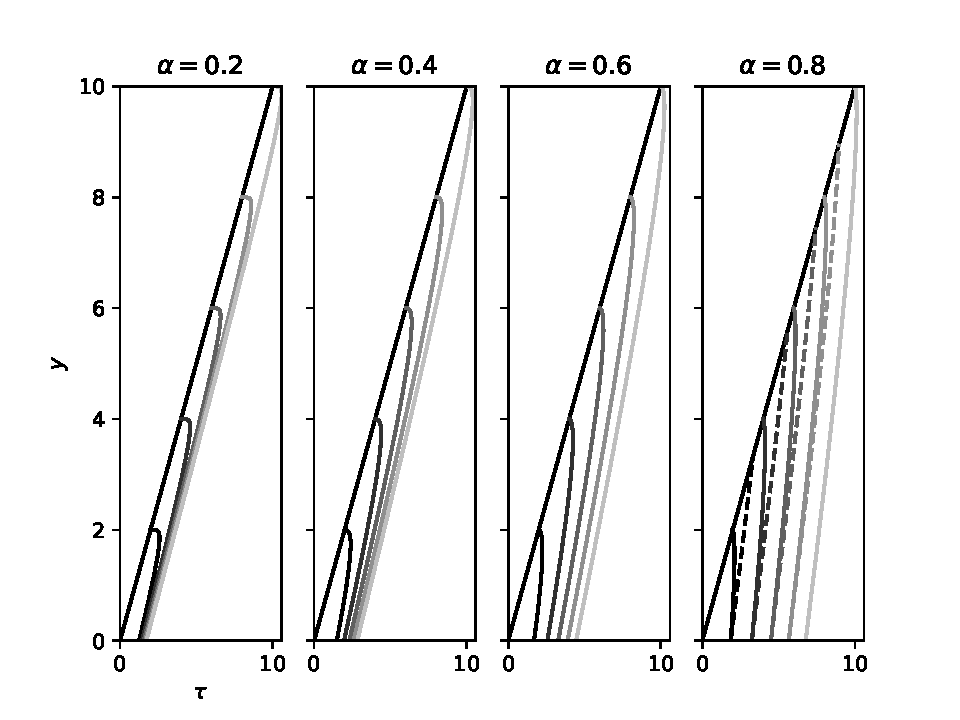
\includegraphics[width=1\textwidth]{geo_int1.pdf}
\caption{A plot of $\Gamma(x)$. $\Gamma(x)$ is not defined for the non-negative integers.}
\label{fig:geo1}
\end{figure}

\begin{figure}[htb]
\centering
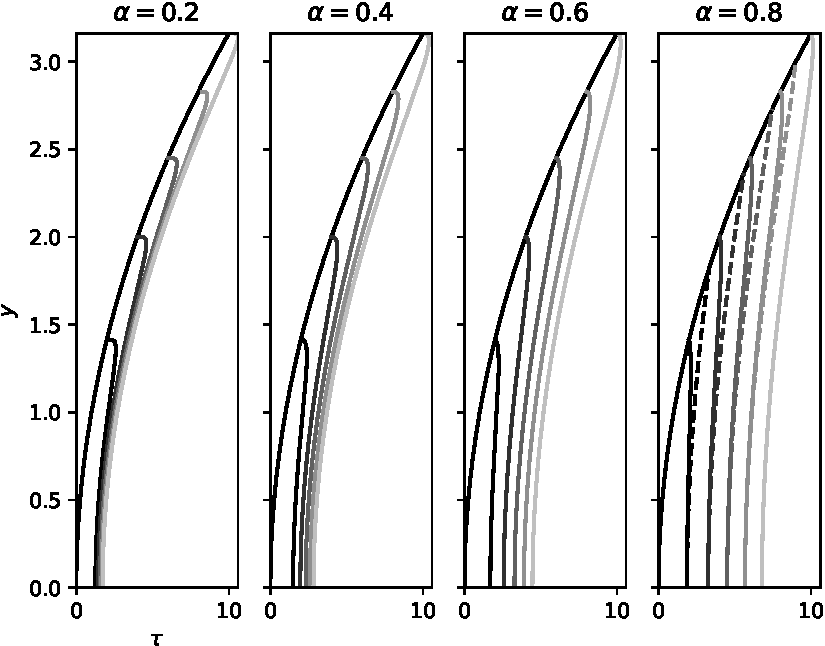
\includegraphics[width=1\textwidth]{geo_int2.pdf}
\caption{A plot of $\Gamma(x)$. $\Gamma(x)$ is not defined for the non-negative integers.}
\label{fig:geo2}
\end{figure}



These steps 
were discussed in more detail in the previous section. 

The steps to visualize the above two integrals were described in the previous paragraph. We first convert the integrals into Riemann-Stieltjes integrals. The 
Riemann-Stieltjes integrals are then converted to Cavalieri integrals. We can then simply depict the Cavalieri integrals and in doing so obtain a geometric interpretaion
of the original fractional integrals. Importantly, for each value of $t$ we obtain a different 








\section{First-level section heading}

Section headings use an initial capital letter on the first word, with subsequent words lowercase.  In general, the style of the journal is to leave all section headings unnumbered.  Consult the journal editor if you wish to depart from this and other conventions.

\subsection{Second-level heading}

The same goes for second-level headings.  It is not necessary to add font commands to make the math within heads bold and sans serif; this change will occur automatically when the production style is applied.

\section{Graphics}

Figures for the \textsc{Journal} can be submitted as either color or black \& white graphics.  Generally, color graphics will be used for the online publication, and converted to black \& white images for the print journal.  We recommend using whatever graphics program you are most comfortable with, so long as the submitted graphic is provided as a separate file using a standard file format.

For best results, please follow the following guidelines:
\begin{enumerate}
\item Bitmapped file formats---preferably TIFF or JPEG, but not BMP---are appropriate for photographs, using a resolution of at least 300 dpi at the final scaled size of the image.
\item Line art will reproduce best if provided in vector form, preferably EPS.
\item Alternatively, both photographs and line art can alternatively be provided as PDF files.  Note that creating a PDF does not affect whether the graphic is a bitmap or vector; saving a scanned piece of line art as PDF does not convert it to scalable line art.
\item If you generating graphics using a \TeX\ package, please be sure to provide a PDF of the manuscript.  In the production process, \TeX-generated graphics will eventually be converted to more conventional graphics so the \textsc{Journal} can be delivered in e-reader formats.
\item For photos of contributing authors, we prefer photos that are not cropped tight to the author's profile, so that production staff can crop the head shot to an equal height and width.  If possible, avoid photographs that have excess shadows or glare.
\end{enumerate}

\section{Theorems, definitions, proofs, and all that}

Following the defaults of the \texttt{amsthm} package, styling is provided for \texttt{theorem}, \texttt{definition}, and \texttt{remark} styles, although the latter two use the same styling.

\begin{theorem}[Pythagorean Theorem]
Theorems, lemmas, axioms, and the like are stylized using italicized text. These environments can be numbered or unnumbered, at the author's discretion.
\end{theorem}

\begin{proof}
Proofs set in roman (upright) text, and conclude with an ``end of proof'' (q.e.d.) symbol that is set automatically when you end the proof environment.  When the proof ends with an equation or other non-text element, you need to add \verb~\qedhere~ to the element to set the end of proof symbol; see the \texttt{amsthm} package documentation for more details.
\end{proof}

\begin{definition}[Secant Line]
Definitions, remarks, and notation are stylized as roman text.  They are typically unnumbered, but there are no hard-and-fast rules about numbering.
\end{definition}

\begin{remark}
Remarks stylize the same as definitions.
\end{remark}

Note that the \textit{College Mathematics Journal\/} is meant to be accessible to a broad audience, so heavy use of theorem-like formalisms is generally discouraged.

\begin{acknowledgment}
The authors wish to thank the Greek polymath Anonymous, whose prolific works are an endless source of inspiration.
\end{acknowledgment}

\begin{abstract}
An abstract should not contain concrete mathematics, but rather should be discrete.  Be brief and avoid using mathematical notation except where absolutely necessary, since this brief synopsis will be used by search engines to identify your article!
\end{abstract}

\begin{thebibliography}{1}
\bibitem{parker13} Adam Parker, Who solved the Bernoulli equation and how did they do it? \textit{Coll. Math. J.} \textbf{44} (2013) 89--97.

\bibitem{hopkins} Brian Hopkins, ed., \textit{Resources for Teaching Discrete Mathematics}, Mathematical Association of America, Washington DC, 2009.
\end{thebibliography}
\vfill\eject

\end{document}
